\documentclass{standalone}
\usepackage{tikz}
\usetikzlibrary{shapes,arrows,calc,positioning,decorations.markings,shadows}
\usepackage{amsmath,amsfonts,graphicx,pgfplots}
\begin{document}

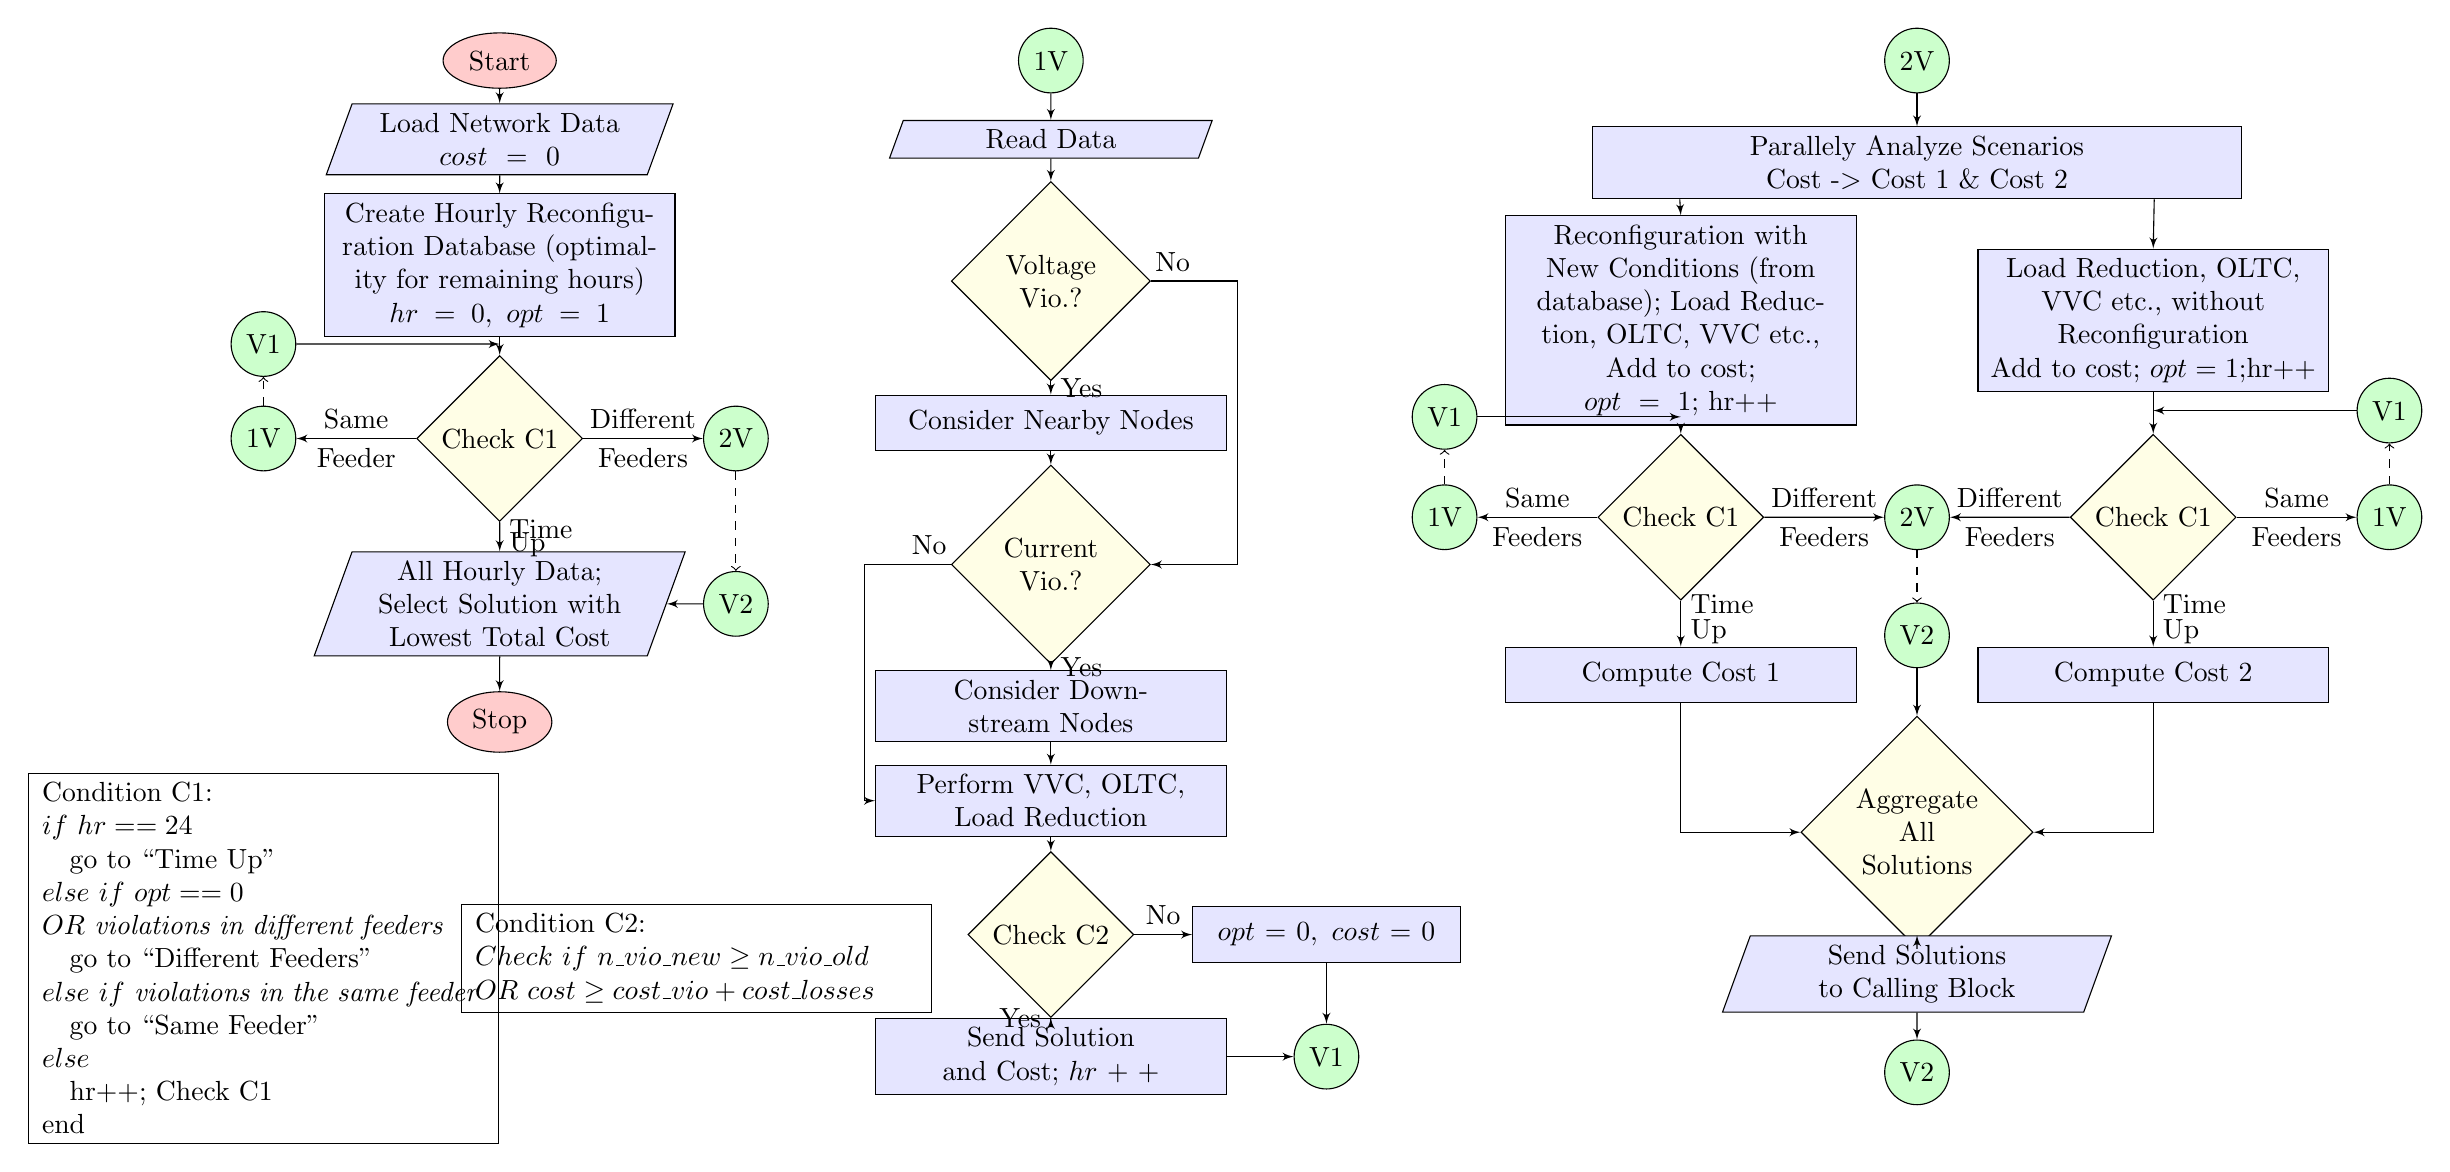
\begin{tikzpicture}[node distance = 1.5cm, auto]
%\scriptsize

	% Define block styles
	\tikzstyle{decision} = [diamond, draw, fill=yellow!10, 
    text width=4.5em, text badly centered, node distance=3cm, inner sep=2pt]
	\tikzstyle{block} = [rectangle, draw, fill=blue!10, 
    text width=12em, text centered, minimum height=2em, minimum width=12em]
	\tikzstyle{io} = [trapezium, trapezium left angle=70, trapezium right angle=110, text centered, text width=10em, minimum width=10em, draw, fill=blue!10]
	\tikzstyle{line} = [draw, -latex']
	\tikzstyle{cloud} = [draw, ellipse,fill=red!20, node distance=3cm,
    minimum height=2em]
	\tikzstyle{con} = [draw, circle,fill=green!20, node distance=3cm,
    minimum height=2em]
	\tikzstyle{blank} = [node distance=1cm,minimum width=-1cm]
	\tikzstyle{legend} = [rectangle, draw,
    text width=16em, minimum height=2em, minimum width=17em]

	% Main Flow Chart
	\node [blank] (start) {};
	\node [cloud, below of=start, node distance=0cm] (init) {Start};
   	\node [io, below of=init, node distance=1cm] (load) {Load Network Data\\$cost=0$};
	\node [block, below of=load, node distance=1.6cm] (rec1) {Create Hourly Reconfiguration Database (optimality for remaining hours)\\ $hr=0,\ opt=1$};
	\node [decision, below of=rec1, node distance=2.2cm] (check1) {Check C1};
	\node [blank, below of=rec1,node distance=1.0cm] (b1) {};
	\node [con, left of=b1] (V1_1) {V1};
	\node [con, left of=check1] (1V_1) {1V};
	\node [con, right of=check1] (2V_1) {2V};
	\node [con, below of=2V_1, node distance=2.1cm] (V2_1) {V2};
	\node [blank, below of=check1] (b2) {};
	\node [io, below of=check1, node distance=2.1cm] (fin1) {All Hourly Data;\\Select Solution with Lowest Total Cost};
	\node [cloud, below of=fin1, node distance=1.5cm] (stop) {Stop};

	% Main Flowchart Paths
	\path [line] (init) -- (load);
	\path [line] (load) -- (rec1);
	\path [line] (rec1) -- (check1);
	\path [line] (V1_1) -- ($(b1.east)!0.5!(b1.west)$);
	\path [line] (check1.west) -- node [yshift=1.4em]  {Same} node {Feeder} (1V_1);
	\draw[dashed,->] (1V_1) -- (V1_1);
	\path [line] (check1.east) -- node {Different} node  [yshift=-1.4em] {Feeders} (2V_1);
	\path [line] (V2_1) -- (fin1);
	\draw[dashed,->] (2V_1) -- (V2_1);
	\path [line] (check1) -- node [near start] {Time} node [yshift=-0.3em] {Up} (fin1);
	\path [line] (fin1) -- (stop);

	% V1 Flowchart
	\node [con, right of= start, node distance=7cm](1V) {1V};
	\node [io, below of=1V, node distance=1cm] (read1V) {Read Data};
	\node [decision, below of=read1V, node distance=1.8cm](des1V_V) {Voltage Vio.?};
	\node [block, below of=des1V_V, node distance=1.8cm] (conV) {Consider Nearby Nodes};
	\node [decision, below of=conV, node distance=1.8cm](des1V_I) {Current Vio.?};
	\node [block, below of=des1V_I, node distance=1.8cm] (conI) {Consider Downstream Nodes};
	\node [block, below of=conI, node distance=1.2cm] (write1V) {Perform VVC, OLTC, Load Reduction};
	\node [decision, below of=write1V, node distance=1.7cm] (ok1V) {Check C2};
	\node [block, right of=ok1V, node distance=3.5cm, minimum width=9em, text width=9em] (no1V) {$opt=0,\ cost = 0$};
	\node [block, below of=ok1V, node distance=1.55cm] (res1V) {Send Solution and Cost; $hr++$};
	\node [con, right of=res1V, node distance=3.5cm] (V1) {V1};

	% V1 Flowchart Paths
	\path [line] (1V) -- (read1V);
	\path [line] (read1V) -- (des1V_V);
	\path [line] (des1V_V) -- node {Yes} (conV);
	\path [line] (des1V_V.east) --  node [near start] {No} +(1.1,0) |- (des1V_I.east);
	\path [line] (conV) -- (des1V_I);
	\path [line] (des1V_I) -- node {Yes} (conI);
	\path [line] (des1V_I.west) --  node [near start,yshift=1.4em] {No} +(-1.1,0) |- (write1V.west);
	\path [line] (conI) -- (write1V);
	\path [line] (write1V) -- (ok1V);
	\path [line] (ok1V) --  node [near start] {Yes} (res1V);
	\path [line] (ok1V) -- node {No} (no1V);
	\path [line] (no1V) -- (V1);
	\path [line] (res1V) -- (V1);

	% V2 Flowchart
	\centering
	\node [con, right of= start, node distance=18cm](2V) {2V};
	\node [block, below of=2V,minimum width=8cm,text width=8cm,node distance=1.3cm] (parallel) {Parallely Analyze Scenarios\\Cost -$>$ Cost 		1 \& Cost 2};
	\node [blank, below of=parallel, node distance=2cm] (bx) {};
	\node [block, left of=bx, node distance=3cm] (reconf) {Reconfiguration with New Conditions (from database); Load Reduction, OLTC, VVC etc.,\\ Add to cost; $opt=1$; hr++};
	\node [block, right of=bx, node distance=3cm] (lrvvc) {Load Reduction, OLTC, VVC etc., without Reconfiguration\\ Add to cost; $opt=1$;hr++};
	\node [blank, below of=reconf, node distance=1.225cm] (b3) {};
	\node [decision, below of=reconf, node distance=2.5cm] (check2) {Check C1};
	\node [con, left of=b3] (V1_2) {V1};
	\node [con, left of=check2] (1V_2) {1V};
	\node [block, below of=check2, node distance=2cm] (C1) {Compute Cost 1};

	\node [con, below of=2V, node distance=5.8cm] (2V_2) {2V};
	\node [con, below of=2V_2, node distance=1.5cm] (V2_2) {V2};
	\node [blank, below of=check2] (b4) {};
	\node [blank, below of=lrvvc, node distance=1.145cm] (b5) {};
	\node [decision, below of=lrvvc, node distance=2.5cm] (check3) {Check C1};
	\node [con, right of=b5] (V1_3) {V1};
	\node [con, right of=check3] (1V_3) {1V};
	\node [block, below of=check3, node distance=2cm] (C2) {Compute Cost 2};

	\node [decision, below of=parallel, node distance=8.5cm] (check4) {Aggregate All Solutions};
	\node [io, below of=check4, node distance=1.8cm, text width=4cm] (fin2) {Send Solutions to Calling Block};
	\node [con, below of=fin2, node distance=1.25cm] (V2) {V2};
	
	%V2 Flowchart Paths
	\path [line] (2V) -- (parallel);
	\path [line]  ($(parallel.south)!0.7305!(parallel.south west)$) -- (reconf.north);
	\path [line]  ($(parallel.south)!0.7305!(parallel.south east)$) -- (lrvvc.north);
	\path [line] (reconf) -- (check2);
	\path [line] (lrvvc) -- (check3);
	\path [line] (V1_2) -- ($(b3.east)!0.5!(b3.west)$);
	\path [line] (V1_3) -- ($(b5.east)!0.5!(b5.west)$);
	\path [line] (check2.east) -- node {Different} node  [yshift=-1.4em] {Feeders} (2V_2);
	\path [line] (check3.west) -- node  [yshift=1.4em] {Different} node {Feeders} (2V_2);
	\path [line] (V2_2) -- (check4);
	\draw[dashed,->] (2V_2) -- (V2_2);
	\path [line] (check2.west) -- node  [yshift=1.4em] {Same} node {Feeders} (1V_2);
	\path [line] (check3.east) -- node {Same} node  [yshift=-1.4em] {Feeders} (1V_3);
	\draw[dashed,->] (1V_2) -- (V1_2);
	\draw[dashed,->] (1V_3) -- (V1_3);
	\path [line] (check2) --  node [near start, yshift=0.3em] {Time} node [yshift=-0.3em] {Up} (C1);
	\path [line] (check3) --  node [near start, yshift=0.3em] {Time} node [yshift=-0.3em] {Up} (C2);
	\path [line] (C2.south) |- (check4.east);
	\path [line] (C1.south) |- (check4.west);
	\path [line] (check4.south) -- (fin2);
	\path [line] (fin2) -- (V2);

	% Legend
	\node [blank, below of=stop, node distance=3cm] (bleg) {};
	\node [legend, left of=bleg, node distance=3cm] (leg) {Condition C1:\\$if\ hr == 24$\\\ \ \ go to ``Time Up''\\$else\ if\ opt == 0$\\$OR$ \textit{violations in different feeders}\\\ \ \ go to ``Different Feeders''\\$else\ if$ \textit{violations in the same feeder}\\\ \ \ go to ``Same Feeder''\\$else$\\\ \ \ hr++; Check C1\\end};
	\node [legend, right of=bleg, node distance=2.5cm] (leg1) {Condition C2:\\$Check\ if\ n\_vio\_new \ge n\_vio\_old$\\$OR\ cost \ge cost\_vio+cost\_losses$};

\end{tikzpicture}

\end{document}